% Die Architektur wurde erfolgleich angewendet
Die dargestellte Architektur und deren Regeln lassen sich gut bei der Umsetzung der Aufgabe anwenden 
und dienen auch als Dokumenation zu den Anwendungen. Anhand dieser Architektur lässt sich der Schnittpunkt zweier Geraden 
aus der Abbildung \ref{fig:softQuality} nach Links auf der Zeitachse verschieben (siehe nachfolgende Abbildung),
indem es deutlich weniger Entscheidungen getroffen werden müssen und somit können kleine Projekte 
gute Qualität besitzen.

\begin{figure}[H]
    \centering
    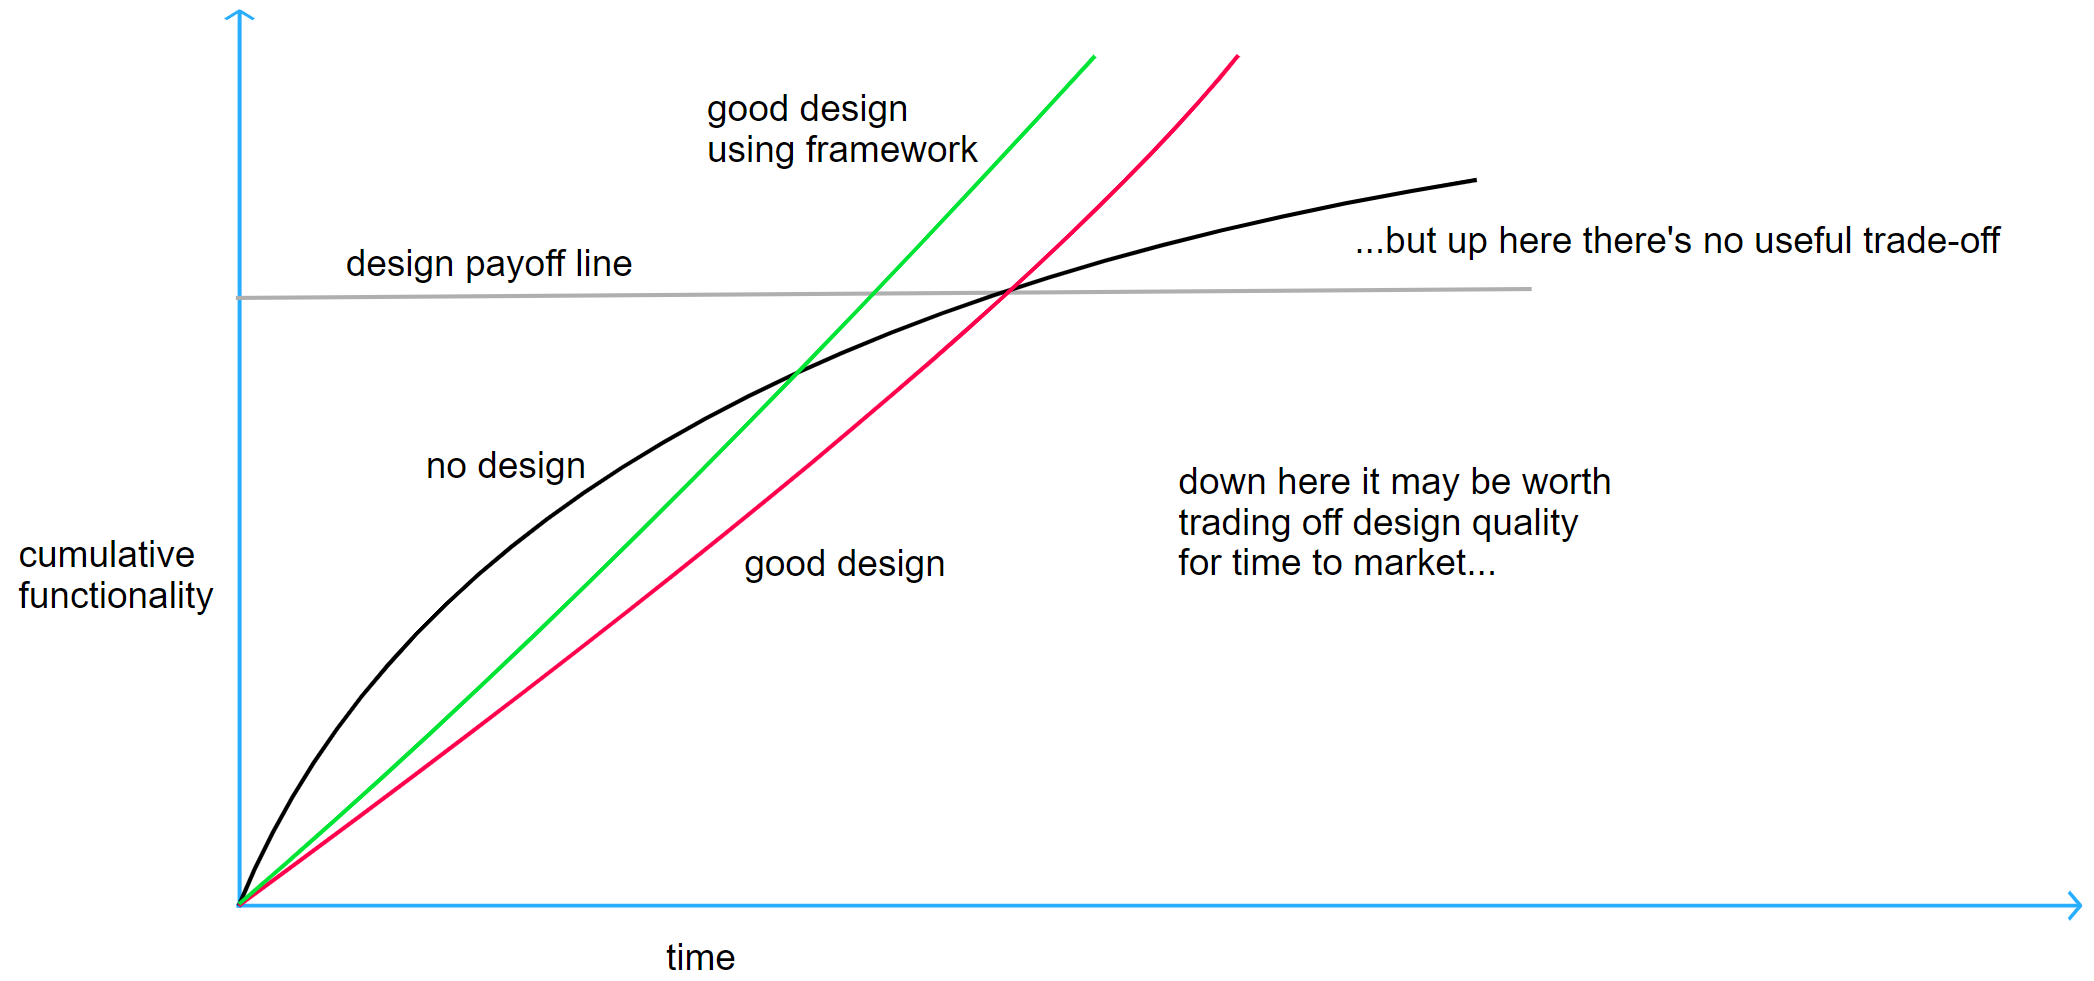
\includegraphics[width=1\textwidth]{./images/QASoftwareCompareWithFramework.png}
    \caption[Verwendung der Architektur]{Verwendung der Architektur}
    \label{fig:softQualityWithFramework}
\end{figure} 

% Schlussfolgerungen
Eine gut organsierte Architektur hilft bei vielen Problemen, die während der Entwicklung entstehen, 
indem die Lösung bereits allgemein beschrieben ist. 

Der Unterschied zwischen einer Bibliothek und einem Framework besteht nur an der vorgegebene Schnittstelle, 
die die Möglichkeiten das Verhalten der Anwendung zu ändern begrenzt. 
Alle Anwendungen besitzen den gleichen Kern, der aus unterschiedlichen Implementationen von \textbf{Ports} und \textbf{Adapters} besteht.
Der Kern wird in der Schnittstelle (im Falle einer Bibliothek und eines Frameworks) oder im Hauptprogramm (im Falle einer Standalone-Anwendung) gebaut.


% Ergebnis an Codezeilen vergleichen, Anzahl an Unittests
In der nachfolgenden Tabelle werden vier Lösungen jeweils miteinander verglichen.
In den Zellen werden gemeinsame Codezeilen von zwei Anwendungen abgebildet.
Anzahl an gemeinsame Codezeilen für alle Projekte ist 25.799 (entspricht Abbildung \ref{fig:commonPartOfEverySolution}). 
\begin{table}[h!]
    \centering
    \begin{tabular}{|c|c| c| c| c| }
    \hline
                        & Standalone mit DB & Standalone ohne DB    & Framework & Library \\ 
    \hline
    Standalone mit DB   & 28.466             &                       &           & \\  
    \hline
    Standalone ohne DB  & 26.210             & 26.417                 &           & \\  
    \hline
    Framework           & 25.799             & 25.972                 & 26.888     & \\  
    \hline
    Library             & 25.799             & 25.972                 & 25.799     & 26.112 \\
    \hline
    \end{tabular}
    \caption{Vergleich der Anzahl der Codezeilen}
    \label{tab:compareLoC}
\end{table}

\newpage
Durch die Anwendung von Tests ließ sich die Entwicklung beschleunigen, indem die Fehler gleich angezeigt wurden.
In der nachfolgenden Tabelle \ref{tab:compareTests} ist die Verteilung des Tests zu sehen, 
die der Verteilung in der ``Testing Pyramide'' (siehe Kapitel \ref{kap:testingPyramide}) entspricht. 
Die automatisieren Tests in den Anwendungen sind wie folgt verteilt:

\begin{table}[h!]
    \centering
    \begin{tabular}{|c|c|c|c|c|}
        \hline
                & Unittests & Integrationtests & Systemtests & UI-Tests \\
        \hline
        Anzahl  & etwa 650  & etwa 150  & 2  & UI ist nicht vorhanden \\  
        \hline
    \end{tabular}
    \caption{Darstellung an automatisierten Tests}
    \label{tab:compareTests}
\end{table}

\subsection{Ausblick}
Die im Kapitel \ref{kap:commonArchitectureDescription} dargestellte Architektur 
lässt sich auch auf andere Applikationen anwenden. 
Dazu zählen neben den Monolith-Anwendungen die Mikroservices-, Desktop- und Embedded-Anwendungen.
Weiterführend kann noch Parallelismus betrachtet werden, 
das bessere Verwendung der vorhandenen Ressourcen und die Skalierung der Anwendung ermöglicht.

% umschreiben, mehr schreiben
Im Kapitel \ref{kap:commonArchitectureDescription} werden viele Regeln und Eigenschaften der Architektur allgemein dargestellt, 
indem viele Abläufe, Datentransformationen und Teile der Architektur beschrieben sind.
Durch die Flexibilität und Unabhängigkeit der Architektur besitzen die Anwendungen, die mittels dieser Architektur umgesetzt sind, viele Gemeinsamkeiten.
Diese Gemeinsamkeiten müssten bei der Nutzung der Architektur immer neu umgesetzt werden.
Bei der Umsetzung wird die Zeit benötigt und es können auch Fehler in der Architektur entstehen, indem nicht alle Regeln bzw. Vorgaben eingehalten werden.
Das lässt sich mittels eines Frameworks vermeiden, das die gemeinsamen Teile wie Code, Struktur und Datenfluss,  
und Eigenschaften wie Testbarkeit, Erweiterbarkeit und Änderbarkeit vorgibt bzw. mit sich bringt.
Das Framework kann somit eine Grundlage für viele andere Projekte sein, 
die dadurch schneller umgesetzt werden und bessere Qualität besitzen.
Durch die Nutzung dieses Frameworks können die Softwareteams flexibel sein,
weil alle Projekte die gleiche Struktur besitzen und somit wird die Einarbeitungszeit von neuen Mitarbeitern reduziert.

\begin{figure}[H]
    \centering
    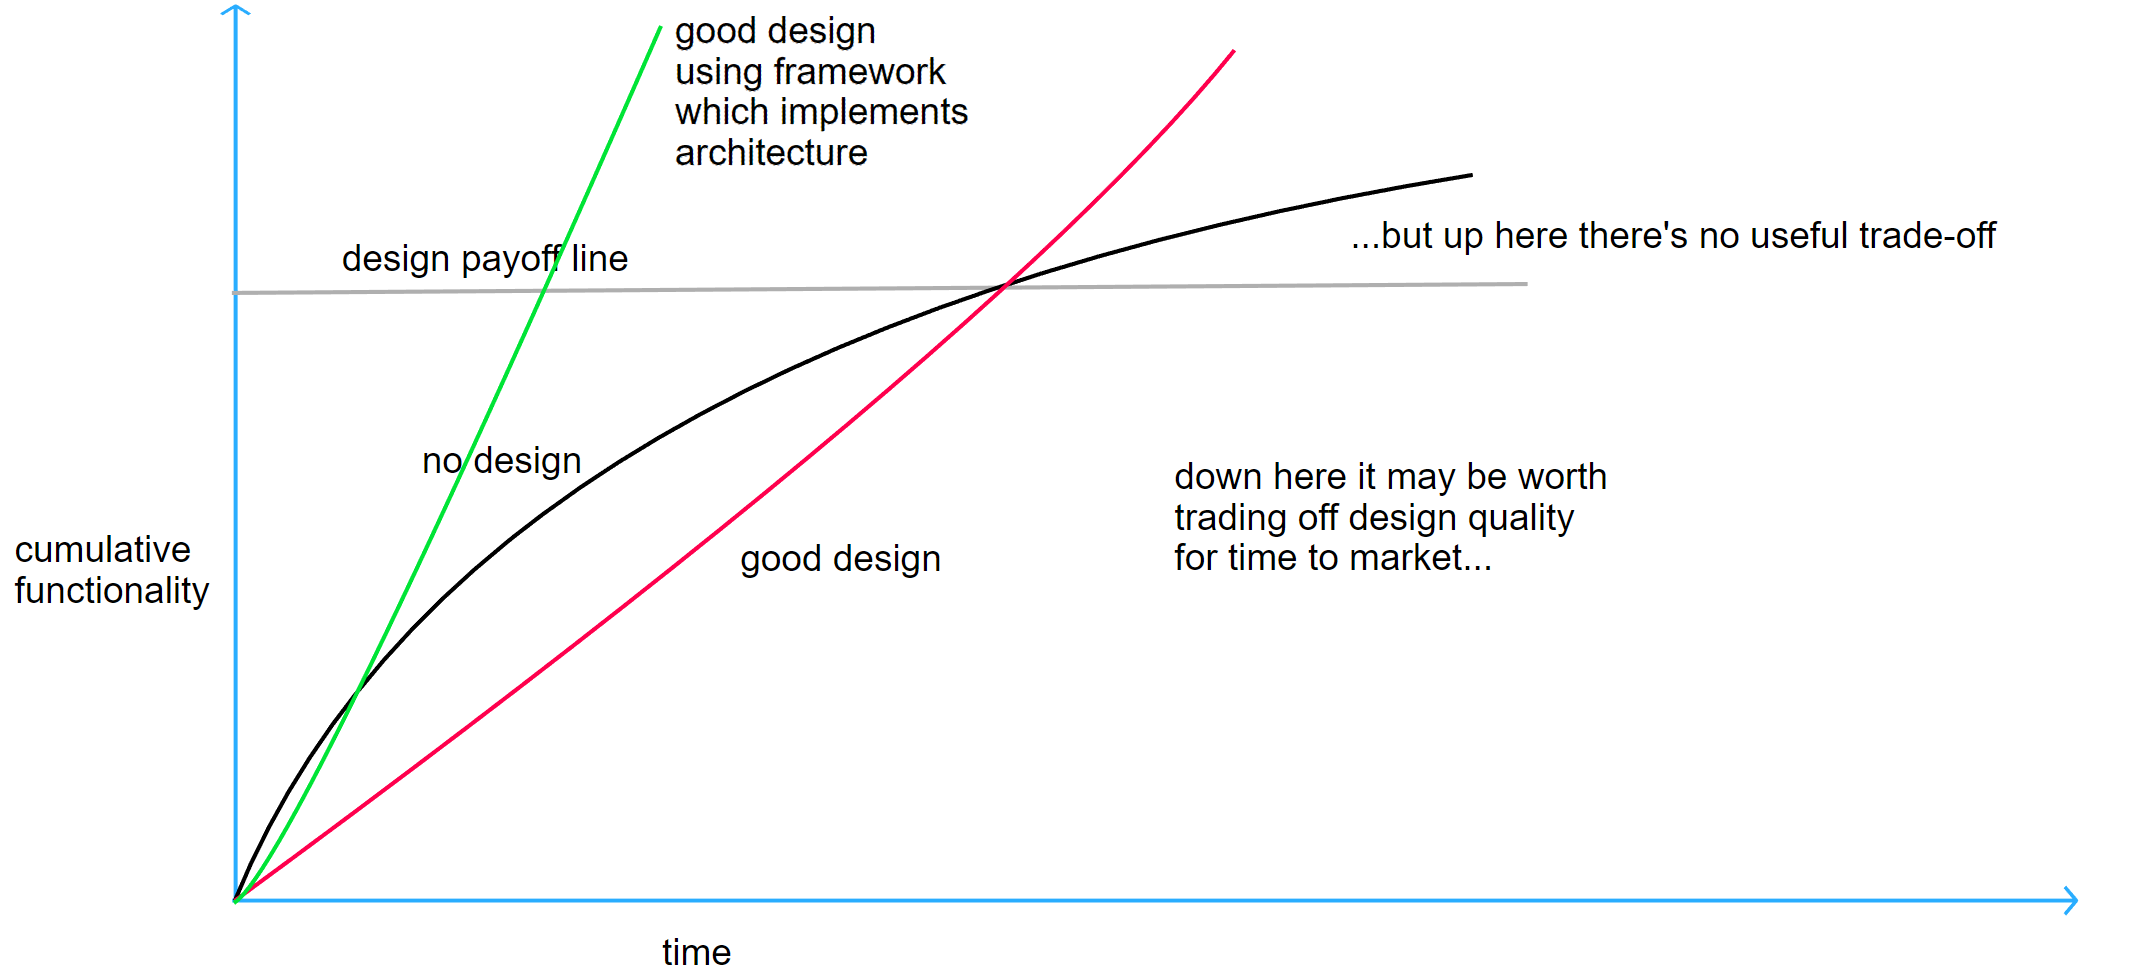
\includegraphics[width=1\textwidth]{./images/QASoftwareCompareWithFramework2.png}
    \caption[Verwendung des Frameworks]{Verwendung des Frameworks}
    \label{fig:softQualityWithFramework2}
\end{figure} 